\begin{frame}
    \frametitle{Wstęp}

    Rozdziały pracy:
    \begin{enumerate}
        \item Podstawowe definicje teorii grafów
        \item Uczenie maszynowe
        \item Wykorzystywane technologie
        \item Opis modelu podstawowego
        \item Testy
    \end{enumerate}

\end{frame}

\begin{frame}
    \frametitle{Wstęp}

    \begin{figure}[ht]
        \centering
        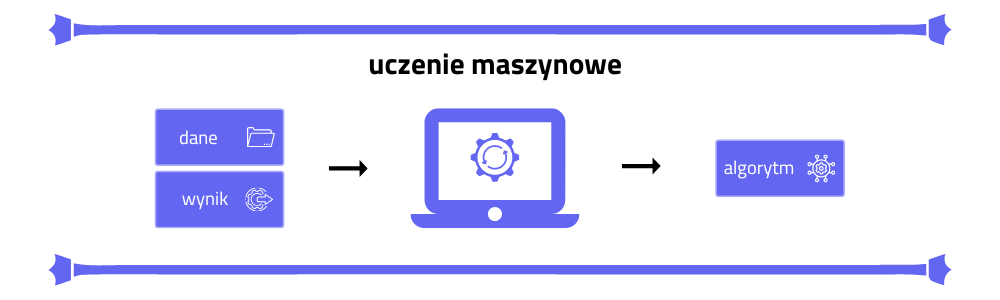
\includegraphics[width=\textwidth]{resources/img/przerywnik-machine-learning.png}
        \caption{Wizualizacja konceptu uczenia maszynowego.
		    Źródło: https://bluemetrica.com/czym-jest-machine-learning}
    \end{figure}

\end{frame}